\documentclass[a4paper]{article}

% Packages
\usepackage{amsmath}
\usepackage{amssymb}
\usepackage{amsthm}
\usepackage{bold-extra}
\usepackage{fancyhdr}
\usepackage{geometry}
\usepackage{graphicx}
\usepackage{hyperref}
\usepackage{ifthen}
\usepackage[utf8]{inputenc}
\usepackage{multirow}
\usepackage{needspace}
\usepackage{parskip}
\usepackage{stmaryrd}
\usepackage{listings}
\usepackage[T1]{fontenc}
\usepackage{longtable}
\usepackage{comment}
\usepackage{enumerate}
\usepackage{xspace}
\usepackage{textcomp}
\usepackage{array}

\usepackage{tikz}
\usetikzlibrary{automata,positioning,shapes.geometric}
\usepackage{tikzsymbols}
\usepackage{todonotes}

\lstset{language=Java, numbers=left, showstringspaces=false, tabsize=4}
\geometry{a4paper, left=25mm,right=25mm, top=25mm, bottom=25mm}

% check for the existence of commands
\newcommand{\checkfor}[3]{%
  \ifcsname#1\endcsname%
  #2
  \else%
  #3
  \fi%
}

\checkfor{exnumber}{}{\newcommand{\exnumber}{-1}}

\newcommand{\exercisepagebreak}{\checkfor{isexercise}{\pagebreak}{}}
\newcommand{\solutionpagebreak}{\checkfor{isexercise}{}{\pagebreak}}

\setcounter{section}{\exnumber{}}

\numberwithin{equation}{section}
\numberwithin{figure}{section}
\numberwithin{table}{section}
\renewcommand{\qedsymbol}{\textsc{q.e.d.}}
\renewenvironment{proof}[1][\proofname]{{\bfseries #1: }}{\qed}
\newtheoremstyle{defstyle}{10pt}{5pt}{\addtolength{\leftskip}{2\leftmargini}\addtolength{\rightskip}{2\leftmargini}}{-1\leftmargini}{\scshape\bfseries}{:}{\newline}{#1 #2\ifthenelse {\equal {#3}{}} {}{ (\text{\textsc{#3}})}}{}
\newtheoremstyle{thmstyle}{10pt}{5pt}{\addtolength{\leftskip}{2\leftmargini}\addtolength{\rightskip}{2\leftmargini} \slshape}{-1\leftmargini}{\scshape\bfseries}{:}{\newline}{#1 #2\ifthenelse {\equal {#3}{}} {}{ (\text{\textsc{#3}})}}{}
\newtheoremstyle{exstyle}{10pt}{5pt}{\addtolength{\leftskip}{2\leftmargini}\addtolength{\rightskip}{2\leftmargini}}{-1\leftmargini}{\scshape\bfseries}{:}{\newline}{#1 #2\ifthenelse {\equal {#3}{}} {}{ (\text{\textsc{#3}})}}{}
\newtheoremstyle{algostyle}{10pt}{5pt}{\addtolength{\leftskip}{2\leftmargini}\addtolength{\rightskip}{2\leftmargini}}{-1\leftmargini}{\scshape\bfseries}{:}{\newline}{#1\ifthenelse {\equal {#3}{}} { #2}{ \text{\textsc{#3}}}}{}
\theoremstyle{defstyle}
\newtheorem{mydef}{Definition}[section]
\theoremstyle{thmstyle}
\newtheorem{mythm}{Theorem}[section]
\newtheorem{mylem}[mythm]{Lemma}
\newtheorem{myprop}[mythm]{Proposition}
\theoremstyle{exstyle}
\newtheorem{myex}{Example}[section]
\theoremstyle{algostyle}
\newtheorem{myalgo}{Algorithm}

% Define programming and solution environment and only use if enabled
\checkfor{isprog}{
  % Define exercise environment
  \newcounter{exercise}
  \newenvironment{exercise}[1]{\refstepcounter{exercise}\label{ex\theexercise}\section*{Programming Exercise \theexercise \hfill (#1 Points)}}{}
  \checkfor{isexercise}{
    % Programming exercise
    \excludecomment{solution}
    \excludecomment{onlysolution}
    \newenvironment{onlyexercise}{}{}
    \newcommand{\extitle}{Programming Exercise}
  }{
    % Programming solution
    \newenvironment{solution}{\label{sol\theexercise}\subsection*{Solution: \hrulefill}}{}
    \newenvironment{onlysolution}{}{}
    \excludecomment{onlyexercise}
    \newcommand{\extitle}{Programming Solution}
    }
}{
  % Define exercise environment
  \newcounter{exercise}
  \newenvironment{exercise}[1]{\refstepcounter{exercise}\label{ex\theexercise}\section*{Exercise \theexercise \hfill (#1 Points)}}{}
  \checkfor{isexercise}{
    % Theoretical exercise
    \excludecomment{solution}
    \excludecomment{onlysolution}
    \newenvironment{onlyexercise}{}{}
    \newcommand{\extitle}{Exercise Sheet}
  }{
    % Theoretical solution
    \newenvironment{solution}{\label{sol\theexercise}\subsection*{Solution: \hrulefill}}{}
    \newenvironment{onlysolution}{}{}
    \excludecomment{onlyexercise}
    \newcommand{\extitle}{Solution}
  }
}

% Define header
\pagestyle{fancy}
\fancyhf{} % Clear all headers
\setlength{\headsep}{25pt}
\cfoot{\thepage} % Page numbers
\lhead{ % Header-Definition
  % Logo
  \begin{tabular}[b]{l l}
      \multirow{2}{38mm}{
        \raisebox{-3.6mm}[0pt][0pt]{
          
\includegraphics[height=14mm]{../i2}
        }
      }
      & Lehrstuhl f{\"u}r Informatik 2 \\
      & Software Modeling and Verification
    \end{tabular}
}
\rhead{ % Header-Definition
  % Course name
  \begin{tabular}[b]{r}
    Compiler Construction 2025\\
    \extitle{} \exnumber
  \end{tabular}
}
\AtBeginDocument{
  \vspace*{-30pt}
  apl.\ Prof.\ Dr.\ Thomas Noll\hfill Daniel Zilken, Roy Hermanns
  \vspace{5mm}
}


\newcommand{\header}[1]{
  % Header
  \begin{center}
    {\huge \textbf{Compiler Construction 2025}}\\
    \vspace*{1\baselineskip}%
    {\huge \textbf{--- \extitle{} \exnumber{} ---}}\\
    \checkfor{isexercise}{
      \vspace*{1\baselineskip}
      \checkfor{isprog}{
        %Upload in Moodle until #1 before the exercise class.
      }{
        Upload in Moodle or hand in until #1 before the exercise class.
      }
    }{}
    \vspace*{1.5\baselineskip}
    \hrule
  \end{center}
}

% Change numbering to (a) and (i)
\renewcommand{\labelenumi}{(\alph{enumi})}
\renewcommand{\labelenumii}{(\roman{enumii})}

% Custom commands
\newcommand{\TODO}[1]{\color{red}\textbf{TODO:} #1\color{black}}

% Macros
\newcommand{\set}[1]{\ensuremath{\left\{ #1 \right\}}}
\newcommand{\Nats}{\ensuremath{\mathbb{N}}}
\newcommand{\Reals}{\ensuremath{\mathbb{R}}}

\newcommand{\PTIME}{\mbox{\rm PTIME}}
\newcommand{\PSPACE}{\mbox{\rm PSPACE}}
\newcommand{\coNP}{\mbox{\rm coNP}}
\newcommand{\NP}{\mbox{\rm NP}}
\newcommand{\poly}{\mbox{\rm poly}}
\newcommand{\coPTIME}{\mbox{\rm coPTIME}}
\newcommand{\coPSPACE}{\mbox{\rm coPSPACE}}
\newcommand{\NPSPACE}{\mbox{\rm NPSPACE}}
\def\EXPTIME{\text{\rm EXPTIME}}
\def\doubleEXPTIME{\text{\rm 2EXPTIME}}

% Lecture specific commands
\renewcommand{\L}{{\cal L}}
\newcommand{\numberone}{\ensuremath{\set{1, \dots, 9}}}
\newcommand{\numberzero}{\ensuremath{\set{0, \dots, 9}}}
\newcommand{\eps}{\ensuremath{\varepsilon}}
\newcommand{\sem}[1]{\llbracket#1\rrbracket}
\newcommand{\la}{\ensuremath{\textsf{la}}}
\newcommand{\fir}{\ensuremath{\textsf{fi}}}
\newcommand{\first}{\ensuremath{\textsf{first}}}
\newcommand{\fo}{\ensuremath{\textsf{fo}}}
\newcommand{\follow}{\ensuremath{\textsf{follow}}}
\newcommand{\cyl}[1]{\ensuremath{\mathit{Cyl}(#1)}}
\newcommand{\icompiler}[0]{\texttt{i2Compiler}}
\newcommand{\while}[0]{\textit{WHILE}\xspace}



\begin{document}

\begin{center}
  {\huge \textbf{Compiler Construction 2020/21}}\\
  \vspace*{1\baselineskip}%
  {\huge \textbf{--- \extitle{} \exnumber{} ---}}\\
  \vspace*{1.5\baselineskip}
  \hrule
\end{center}

\begin{onlysolution}
  \begin{center}
    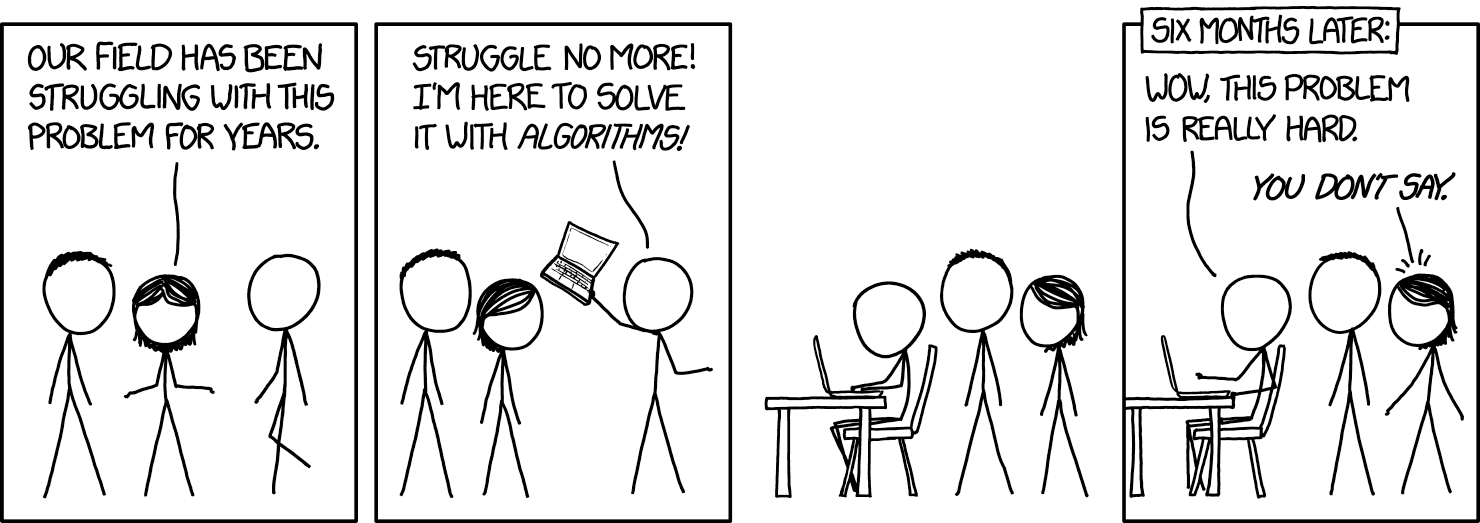
\includegraphics[scale=0.25]{xkcd_algorithms}

    \scriptsize Credit: \href{https://xkcd.com/1831/}{https://xkcd.com/1831/}
  \end{center}
\end{onlysolution}

\section*{General Remarks}
\begin{itemize}
	\item Exercises are \emph{optional}, i.e., not required for admission to exams. However, corrections to students’ solutions are provided as annotations to the submissions.
	%
    \item Please use the corresponding task in the Moodle room to submit your solution. Paper submissions are not accepted.
    %
    \item Please hand in your solutions in \emph{groups of four} and hand in only one solution per group. You can use the forum in this Moodle room to find group members.
\end{itemize}

\begin{exercise}{0}
  Which of the following statements hold?
  \begin{enumerate}
    \item Deterministic finite automata (DFA) are strictly less expressive than regular expressions.
    \item Non-deterministic finite automata (NFA) are strictly more expressive than DFA.
    \item The regular languages are closed under:
      \begin{enumerate}
    	 \item union,
    	 \item intersection,
    	 \item complement,
    	 \item concatenation,
    	 \item Kleene closure.
       \end{enumerate}
    \item Context Free Languages (CFL) are closed under:
      \begin{enumerate}
        \item union,
    	\item intersection,
    	\item complement,
    	\item concatenation,
    	\item Kleene closure.
      \end{enumerate}
    \item DCFL is the set of context free languages that are accepted by deterministic push down automata. Is DCFL = CFL?
  \end{enumerate}
\end{exercise}


\begin{solution}
  \begin{enumerate}
    \item No. One can be effectively converted to another.
    \item No. NFA can be converted to a DFA using the powerset construction (Rabin-Scott construction).
    \item Yes for all. Each operation can be implemented by manipulating a DFA or NFA.
    \item Context Free Languages (CFL) are closed under the following:
      \begin{enumerate}
	    \item Yes. $S_1$ and $S_2$ are starting Non-terminal for two Grammar. $S \to S_1 \mid S_2.$
	    \item No. $L_1 = \{a^ib^ic^j \mid i,j\in\mathbb{N}\}$ and $L_2 = \{a^ib^jc^j \mid i,j\in \mathbb{N}\}$
	    \item No. CFLs are closed under union and if they were closed under complement, they would also be closed under intersection.
	    \item Yes.  $S \to S_1  S_2.$
	    \item Yes. Let $S$ be the starting non-terminal. New Grammar $S' \to S S' \mid \varepsilon$.
	\end{enumerate}
    \item No. Just an intuitive example: Palindromes are in CFL but not in DCFL.
  \end{enumerate}
\end{solution}

\begin{exercise}{0}
  \begin{enumerate}
    \item Describe the language of the following regular expression in words:
      \[r= (0+1)^*0(0+1)^*0(0+1)^*.\]
    \item Construct the regular expression for\ldots
      \begin{enumerate}
        \item the set of all strings with at most one pair of consecutive $0$'s and at most one pair of consecutive $1$'s,
        \item the set of all strings with equal number of $0$'s and $1$'s such that no prefix has two more $0$'s than $1$'s nor two more $1$'s than $0$'s.
      \end{enumerate}
    \item Construct a context free grammar (CFG) for a set of strings of $\{(,)\}^*$ such that every string of the set has equal number of left and right parenthesis, and every prefix has at least as many left parenthesis as  right parenthesis.
  \end{enumerate}
\end{exercise}

\begin{solution}
  \begin{enumerate}
    \item The set of all strings containing at least two $0$'s.
    \item
      \begin{enumerate}
        \item The regular expression is: 
        %maybe next time use a different exercise. There is always a problem with this solution.
        %the below solution is using model checking tools proven to be equivalent to the LTL formula 
        % NOT(0 AND X0)W(0 AND X0 AND XGNOT(0 AND X0)) AND NOT(1 AND X1)W(1 AND X1 AND XGNOT(1 AND X1))
        %= ~(00)W(00 & XG~(00)) & ~(11)W(11 & XG~(11))
        %so if the LTL formula corrently models the specification, the regex should also be correct.
          \begin{align*}
          (0+\eps)(10)^*(01)^*(10)^*(1+\eps) \\
          +(0+\eps)(10)^*(01)^*0 \\
          +(1+\eps)(01)^*(10)^*(01)^*(0+\eps) \\
          +(1+\eps)(01)^*(10)^*1 \\
          \end{align*}
	    \item The regular expression is:
          \[(01 + 10)^*\]
      \end{enumerate}
    \item The CFG is:
      \[S \to (\ S \ ) \ S \mid \eps\]
  \end{enumerate}
\end{solution}


\begin{exercise}{0}
  \begin{enumerate}
    \item Let $r$ and $s$ be regular expressions. Consider the set $X$ such that $X = r.X + s$. Under the assumption that the language of $r$ does not contain $\eps$ (i.e., $\eps \not\in L(r)$), find $X$.
    \item
      \begin{enumerate}
        \item Show that the language $L=\{0^{i^2} \ |\ i\in \mathbb{N}\}$ is not regular.
        \item Show that the language $L=\{a^ib^ic^i \ |\ i\in \mathbb{N}\}$ is not a CFL.
      \end{enumerate}
  \end{enumerate}
\end{exercise}

\begin{solution}
  \begin{enumerate}
    \item Guess the solution to be  $r^*s$ (because it feels right).
      \begin{align}\label{arden}
        X = r.X + s\tag{$\star$}
      \end{align}
      By substituting $r^*s$ for $X$ in the equation (\ref{arden}), we observe that $r^*s$ satisfies this property.
      Thus, $L(r^*s)\subseteq L(X)$.
      Translating the equation to the topology of strings,
      \[X = R.X \cup S\]
      where $R=L(r)$ and $S = L(s)$. Let $\eps \not\in L(r)$.
      Suppose the solution of the above equation is $X= R^*S \cup C$, where $R^*S \cap C = \emptyset$. This new set must also satisfy the equation.
      Thus,
      $$R^*S \cup C = R (R^*S \cup C) \cup S = RR^*S \cup RC \cup S = (RR^*S \cup S) \cup RC = R^* S \cup RC$$
      Since $R^*S \cap C = \emptyset$,  $C\subseteq RC$.
      Now we can see why the condition $\eps \not\in R$ is important, mainly $C\subseteq RC$ has no solution for $C$ when $\eps \not\in R$.

      The proof also shows what happens if $\eps \in R$,  $r^*s + c$ is a solution of equation (\ref{arden}) for any $c$.

    \item
      \begin{enumerate}
        \item Let $L$ be regular and $n$ be the integer in the pumping lemma.
          Let $w = 0^{n^2}$. By pumping lemma $w = xyz$ with $|y|\ge 1$, $|xy|\le n$ and $xy^iz$ is in $L$ for all $i$.
          For $i=2$, $n^2 < |xy^2z| \le n^2 + n$. Or $|zy^2z|$ is strictly  between $n^2$ and $(n+1)^2$.
        \item Assume $L$ is defined by a CFG.
          Let $n$ be the pumping integer. We choose a string $z= a^nb^nc^n$. We write $z = uvwxy$.
          By the premises of the pumping lemma $|vwx|\le n$, thus it cannot contain both $a$ and $c$.
          W.l.o.g. assume $vwx$ does not contain $c$.
          If $v=a^kb^l$ or $x=a^kb^l$ then pumping directly leads to a word not in $L$.
          Therefore assume $v=a^k, w=a^lb^p, x=b^q$.
          Then for $i := 2$: $uv^2wx^2y = a^{n+k}b^{n+q}c^n$. Now either $n+k>n$ or $n+q>n$ and therefore $uv^2wx^2y \not \in L$.
      \end{enumerate}
  \end{enumerate}
\end{solution}


\end{document}
